\part{Base de données de graphe de pangénomes}
\label{part:DBpan}
\chapter{Intégration de pangénomes dans une base de données orientées graphe}

L'utilisation des pangénomes dans l'analyse des génomes procaryotes procure de nouvelles perspectives d'analyse et un nouveau point de vue sur les génomes et leur évolution. Au-delà de ça, il est aussi une solution potentielle dans la gestion et la distribution des génomes face à l'augmentation toujours plus forte du nombre de génomes disponible.

Le pangénome est structurellement un graphe contenant l'information concaténé de plusieurs génomes. Il semble donc tout indiqué d'utiliser une structure de base de données reposant sur cette technologie pour intégrer les pangénomes. C'est le travail que nous avons réalisé lors d'une collaboration avec des chercheurs spécialisés en base de données. 

Dans un premier temps, l'idée était de répondre à une problématique de chargement des pangénomes dans les analyses comparées de PANORAMA. Une solution a pu être trouvé lors d'un hackathon, où nous avons intégré plusieurs pangénomes dans une base de données orientée graphe en utilisant le logiciel Neo4j et le langage Cypher. Cette première étape, encourageante, nous a poussé à aller plus loin en améliorant la méthode d'intégration, mais aussi en ajoutant un workflow d'analyse des graphes de pangénome intégrés. De plus, nous avons appliqué cette analyse à un ensemble de pangénomes appartenant aux espèces du groupe ESKAPE. Cette application nous a permis de mettre en évidence l'existence de module partagé, associer à de la résistance aux antibiotiques, entre différentes espèces d'ESKAPE.

Ce travail, présenter lors d'une conférence sur les bases de données orientés graphes, a permis de montrer l'intérêt et la possibilité de stocker les graphes de pangénome dans une base de données adaptés.

\chapter{Article : Integrating Complex Pangenome Graphs}

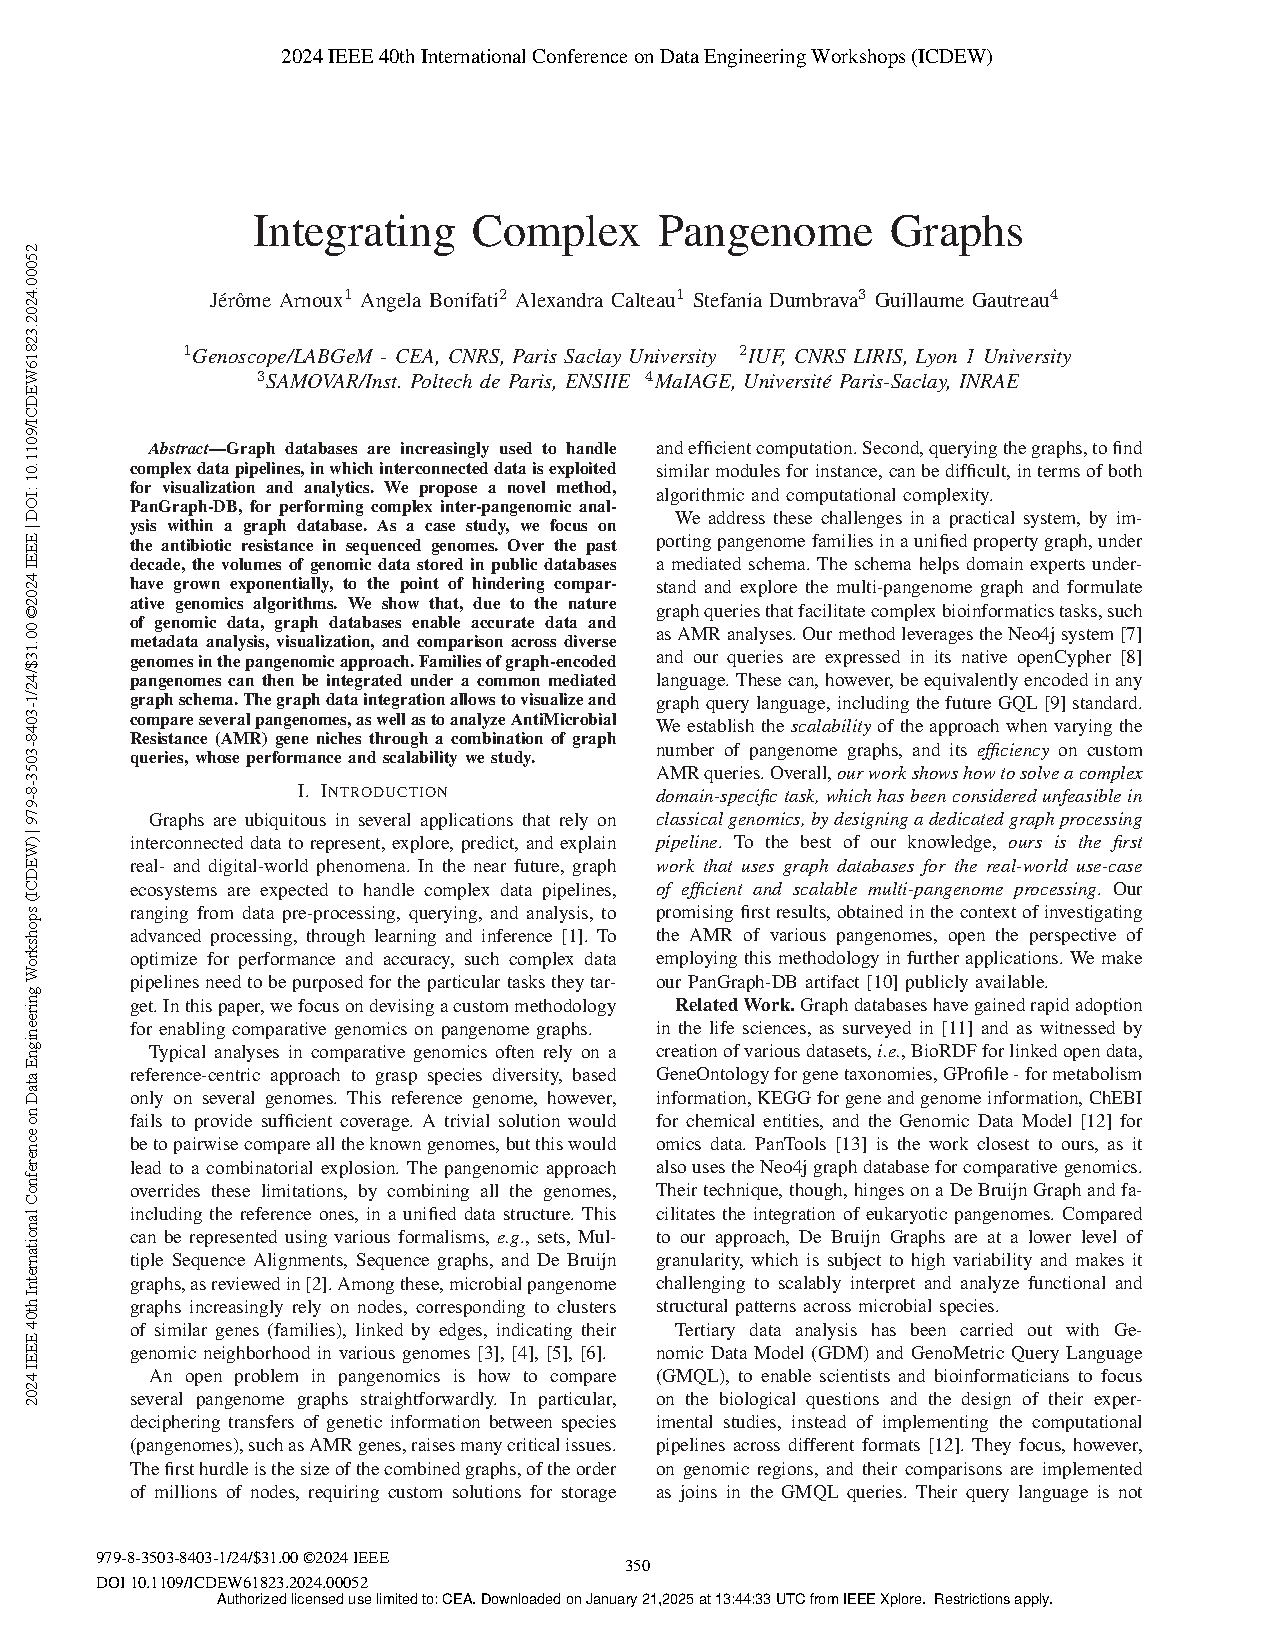
\includepdf[pages=-]{GraphDataBase/Integrating_Complex_Pangenome_Graphs.pdf}

\chapter{Conclusion}

